%!TEX root = ../../csuthesis_main.tex

\chapter{类脑相似性评估与可视化分析}

\section{Brain-Score评估实验设计}

\subsection{测试数据与标准}

为了量化模型与灵长类大脑视觉皮层之间的表征相似性,本文采用Brain-Score提供的公开评估基准进行测试。Brain-Score是由Schrimpf等人提出的类脑模型评估体系,整合了神经电生理记录、人类行为数据和代表性任务表现指标,在神经科学与人工智能领域得到了广泛应用\cite{schrimpf2018brain}。

实验中所使用的神经数据来源于Majaj和Hong等人发布的MajajHong2015公开神经数据集,该数据集记录了两只恒河猴在静态注视条件下,对一组自然图像的皮层响应。图像总数为2560张,全部从ImageNet数据集中筛选,涵盖了64个常见物体类别,如动物、器皿、交通工具等,并经过标准化预处理,包括图像中心对齐、统一灰度背景等操作,以便于神经记录的可比性\cite{majaj2015simple}。

\begin{figure}[!htb]
	\centering
	\begin{subfigure}[t]{0.9\linewidth}
		\centering
		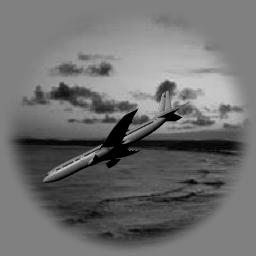
\includegraphics[width=0.25\linewidth]{majaj2015_01.png}
		\hspace{0.05cm}
		
\includegraphics[width=0.25\linewidth]{majaj2015_02.png}
		\hspace{0.05cm}
		
\includegraphics[width=0.25\linewidth]{majaj2015_03.png}
	\end{subfigure}	
	
	\vspace{0.05cm}
	
	\begin{subfigure}[t]{0.9\linewidth}
		\centering
		
\includegraphics[width=0.25\linewidth]{majaj2015_04.png}
		\hspace{0.05cm}
		
\includegraphics[width=0.25\linewidth]{majaj2015_05.png}
		\hspace{0.05cm}
		
\includegraphics[width=0.25\linewidth]{majaj2015_06.png}
	\end{subfigure}
	\caption{MajajHong2015图像示例}
	\label{f.majaj_samples}
\end{figure}

在实验中,研究者使用多电极阵列对恒河猴子的颞下皮层(IT)和视觉皮层第4区(V4)中的数百个神经元通过多电极阵列进行了电生理记录。每张图像呈现约100毫秒,系统记录了神经元在图像呈现后70~170毫秒窗口内的平均响应。V4区主要参与中等复杂度形状与边缘整合,而IT区被认为是高阶语义整合与对象恒常识别的关键区域\cite{dicarlo2012does}。

在神经一致性评估过程中,模型将对与猴子实验中相同的图像集合进行处理,并提取对应层的神经激活。随后,使用偏最小二乘回归(PLS)方法将模型激活映射至神经数据空间,计算皮尔逊相关系数作为匹配度指标,最终得分越高表示模型越“类脑”。这些神经反应数据经过了标准化处理,并由Brain-Score平台封装为benchmark接口,可用于统一评估各类人工视觉模型的神经预测能力。

\subsection{神经区域对齐方式与激活提取策略}

在进行类脑评估实验时,首先需要明确人工神经网络中不同层级的特征表征应如何与大脑视觉皮层中的具体区域进行对应。这一对齐过程是评估神经一致性的基础,也是 Brain-Score 平台设定的关键前提之一。换言之,若模型中间层的输出不能明确映射至生物脑区,则神经预测指标将失去生理解释意义\cite{schrimpf2018brain}。

为了将神经数据与模型结构对应起来,需明确模型中的哪一层特征输出代表生物视觉皮层中的特定脑区。CORnet-Z系列模型具备清晰的模块化分层结构,其V1、V2、V4与IT层模块直接参考了灵长类视觉通路的区域划分。每个模块不仅在结构上模拟了对应脑区的感受野变化和特征抽象过程,还保持了信息传递顺序与神经处理层级一致。因此,该类模型在结构上具有天然的神经对齐优势,广泛用于视觉皮层建模研究中\cite{kubilius2019brain}。

在本实验中,模型的V4模块输出被映射至灵长类大脑的V4区域,IT模块输出则对应真实IT区神经反应。对于每幅图像,模型将输入图像后产生的对应层激活作为表征向量,用于与神经数据进行匹配。激活输出在维度上通过flatten操作转为一维向量,以便参与后续相关性计算。为确保横向比较的公正性,所有待测模型(包括原始CORnet-Z、引入SE模块后的CORnet-Z+SE、加入CBAM模块的CORnet-Z+CBAM,以及将V1替换为VOneBlock的CORnet-Z+VOne)在进行神经一致性评估时均采用相同的激活提取策略与区域对齐方式。

这种模块对脑区的静态映射虽然不能够完全复现真实大脑中存在的多尺度、多方向反馈通路,但在静态图像识别任务中已被多项研究证明具有良好的预测效果。特别是在IT层区域,具备高语义表达能力的深层卷积或递归单元输出,与恒河猴的实际神经响应之间常表现出较高的一致性,是目前类脑建模中最为成熟的区域对齐方式之一\cite{rajalingham2018large}。


\subsection{评估方法与流程}

Brain-Score框架采用神经预测得分(Neural Predictivity)作为主要评估指标,用于衡量模型中间层输出对神经数据的拟合程度。其核心思想是将模型响应与神经反应视为两个向量空间,通过回归拟合和相关性计算判断其相似性。

具体流程如下:

\begin{figure}[hbt]
	\centering
	
\includegraphics[width=0.8\linewidth]{brainscore评估流程图.png}
	\caption{brainscore评估流程图}
	\label{f.brainscore评估流程图}
\end{figure}

图像对齐:所有模型接收与MajajHong2015实验中相同的图像刺激,保持图像顺序、预处理参数与分辨率一致;

激活提取:对每幅图像,提取模型指定层(V4以及IT)的激活向量;

神经预测拟合:通过偏最小二乘回归(PLS)将模型激活映射至神经反应空间,使用皮尔逊相关系数作为拟合度量;

得分计算:对所有神经元的预测得分取平均,作为该层的最终Brain-Score分数,分数范围为0(无关)到1(完美匹配)。

\section{多模型类脑得分对比}

为探究不同结构设计对模型类脑性的影响,本文基于Brain-Score框架,对六种视觉模型在V4和IT两个关键脑区的神经预测能力进行了评估。所测试模型包括:原始CORnet-Z、ResNet-18、AlexNet,以及在CORnet-Z基础上引入三种结构改进的变体(SE模块、CBAM模块、VOneBlock替代V1)。评估指标为Pearson相关系数,表示模型中间层输出与神经实测响应之间的相似性,得分越高,说明模型越“类脑”。

\subsection{在V4脑区的评估结果}

V4区作为腹侧通路的中间阶段,负责对中等复杂度的形状、颜色和边缘特征进行编码。在该区域的评估中,CORnet-Z得分最高(0.5418),紧随其后的是AlexNet(0.5278)与ResNet-18(0.4941)。这三者的共同点在于中前层卷积结构较为浅显,输出激活分布相对广泛,与V4区中神经元对边缘与形状组合的响应特点较为一致。

相比之下,引入注意力机制或生物启发模块的三种改进模型得分均较低,CORnet-Z+SE、CORnet-Z+CBAM、CORnet-Z+VOneBlock分别仅为0.2475、0.2520和0.2213。分析其原因,这些结构在模型内部均强化了特征通道的选择性或稀疏性,改变了中层特征的分布形态。尽管此类机制对分类任务有利,但在与V4区域多通道、非集中响应的神经数据进行匹配时,相关性下降。

在评估过程中,所有模型均以相同预处理流程对图像输入,并在关闭Dropout与BatchNorm更新的推理模式下提取V4层的激活输出。模型输出被转换为一维向量,与大脑神经元反应向量进行对齐。统一的层级命名(如V4.output)使评估系统能直接将模型结构映射至神经区域,排除结构适配偏差。

\begin{figure}[hbt]
	\centering
	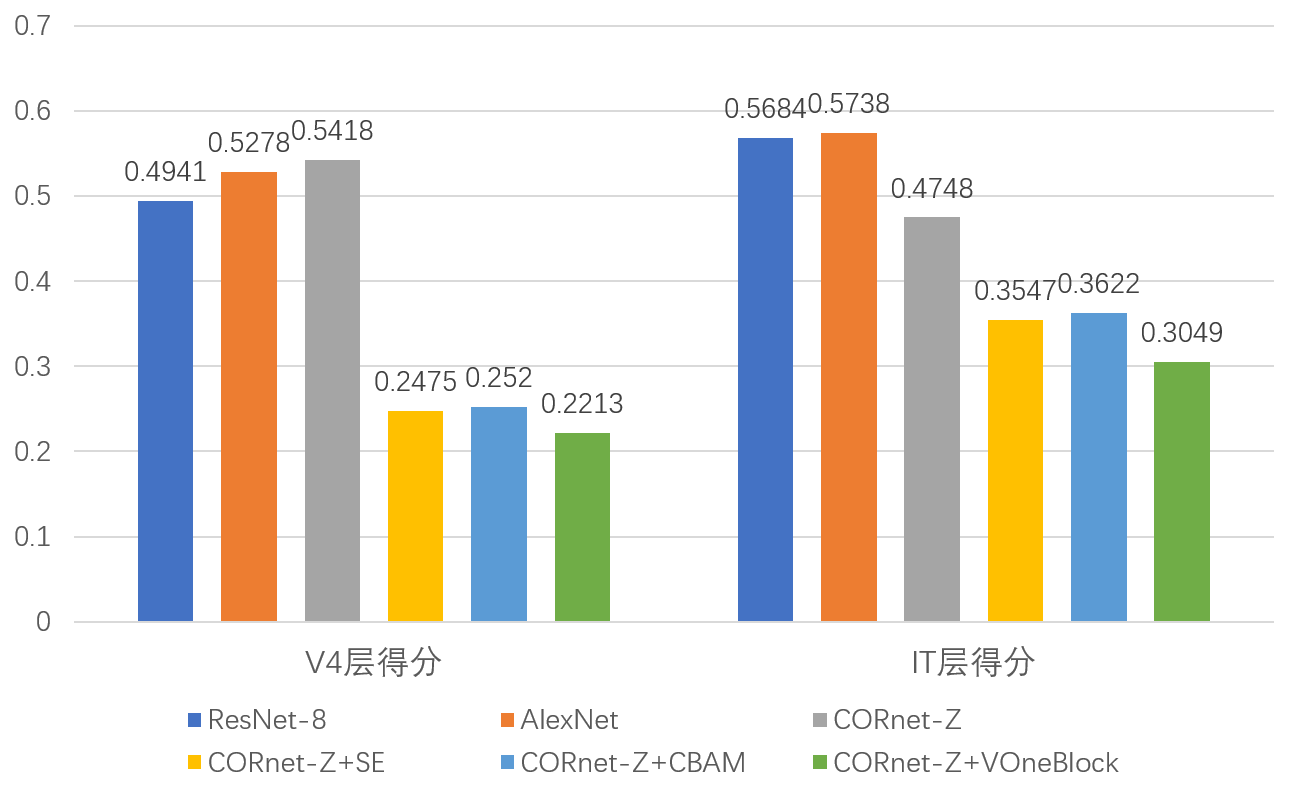
\includegraphics[width=0.8\linewidth]{脑区得分柱状图.png}
	\caption{模型V4与IT脑区得分}
	\label{f.脑区得分柱状图}
\end{figure}

\subsection{在IT脑区的评估结果}

IT区(颞下皮层)是灵长类视觉系统中处理高阶语义的关键脑区,主要编码对象的类别、形状恒常性等抽象信息。在该层的评估中,AlexNet和ResNet-18分别获得了0.5738和0.5684的高分,表现优于其他模型。两者的深层卷积结构和宽激活通道可能更贴近IT区域对丰富语义特征的编码模式。

CORnet-Z模型得分为0.4748,虽然略低于上述两者,但仍优于其三种变体。引入SE模块后的CORnet-Z+SE得分下降至0.3547,CBAM模块略高为0.3622,而将V1层替换为VOneBlock的版本仅为0.3049,说明结构修改带来了更大的激活偏移,影响了对IT神经响应的匹配。

值得注意的是,模型输出经过Brain-Score系统内部的PLS(偏最小二乘回归)拟合,并对每个神经元的预测能力进行评分。最终分数为所有神经元得分的平均值,因此激活的空间范围和通道覆盖度直接影响整体得分表现。部分引入注意力机制的模型,在压缩通道或增强选择性时可能牺牲了多样性,从而导致IT层拟合能力下降。
。

\begin{table}[htb]
	\centering
	\caption{各模型在V4和IT层的类脑评分对比}
	\label{tab:各模型在V4和IT层的类脑评分对比}
	\begin{tabular}{lllll}
		\hline
		模型名称& V4 层得分 & IT 层得分 \\
		\hline
		AlexNet & 0.5278 & 0.5738  \\
		ResNet-18 & 0.4941 & 0.5684  \\
		CORnet-Z & 0.5418 & 0.4748  \\
		CORnet-Z+SE  & 0.2475 & 0.3547  \\
		CORnet-Z+CBMA & 0.2520 & 0.3622  \\
		CORnet-Z+VOneBlock & 0.2213 & 0.3049  \\
		\hline
	\end{tabular}
\end{table}

\subsection{不同结构改进的对比分析}

实验结果表明,不同模型结构的微调对神经一致性得分影响比较显著。在本次实验中,原始的CORnet-Z模型在V4和IT两个脑区都表现出较高的类脑一致性评分,它的结构简洁、模块明确,天然具备较好的神经可映射性。但是,几种基于CORnet-Z模型的结构变体虽然在分类准确率方面略有提升,在Brain-Score指标中却没有体现出更强的神经对齐能力。

为了进一步分析不同结构对模型类脑性能的影响,本文对各模型的关键结构组成进行了整理与比较,如下表所示:

\begin{table}[htb]
	\centering
	\caption{各模型关键结构比较表}
	\label{tab:各模型关键结构比较表}
	\begin{tabular}{lllll}
		\hline
		模型名称& V1层特征处理 & V4层特征处理 & IT层特征处理  \\
		\hline
		CORnet-Z &
		\begin{tabular}[c]{@{}c@{}}Conv7x7+BatchNorm \\+ReLU+MaxPool\end{tabular} &
		\begin{tabular}[c]{@{}c@{}}Conv3x3+BatchNorm \\+ReLU+MaxPool\end{tabular} & \begin{tabular}[c]{@{}c@{}}同V4层\end{tabular} \\
		\hline
		\begin{tabular}[c]{@{}c@{}}CORnet-Z\\+SE\end{tabular} &
		\begin{tabular}[c]{@{}c@{}}Conv7x7+BatchNorm \\+ReLU+MaxPool \\+SE\end{tabular} &
		\begin{tabular}[c]{@{}c@{}}Conv3x3+BatchNorm \\+ReLU+MaxPool \\+SE\end{tabular} & \begin{tabular}[c]{@{}c@{}}同V4层\end{tabular}\\
		\hline
		\begin{tabular}[c]{@{}c@{}}CORnet-Z\\+CBMA\end{tabular} &
		\begin{tabular}[c]{@{}c@{}}Conv7x7+BatchNorm \\+ReLU+MaxPool\end{tabular} &
		\begin{tabular}[c]{@{}c@{}}Conv3x3+BatchNorm \\+ReLU+MaxPool \\+CBMA\end{tabular} & \begin{tabular}[c]{@{}c@{}}同V4层\end{tabular}\\
		\hline
		\begin{tabular}[c]{@{}c@{}}CORnet-Z\\+VOneBlock\end{tabular} &
		\begin{tabular}[c]{@{}c@{}}VOneBlock\\包含Gabor滤波+噪声\end{tabular} &
		\begin{tabular}[c]{@{}c@{}}Conv3x3+BatchNorm \\+ReLU+MaxPool\end{tabular} & \begin{tabular}[c]{@{}c@{}}同V4层\end{tabular} \\
		\hline
	\end{tabular}
\end{table}

这些结构变化虽然增强了模型的表示能力或对某些目标区域的关注能力,但也引入了信息流的重新分布。在类脑评估任务中,模型输出需与灵长类神经反应高度一致,而注意力机制往往会引导模型聚焦于更具判别性的通道,可能牺牲掉部分自然图像中存在的冗余空间信息,这种代价在神经预测任务中表现为得分下降。

结合表~\ref{tab:各模型在V4和IT层的类脑评分对比}中的类脑评分数据,可以发现原始CORnet-Z在V4层和IT层分别取得了0.5418和0.4748的得分,均高于所有结构改进版本。引入SE后,尽管模型在Tiny-ImageNet-200分类任务上的Top-1和Top-5准确率有所提升,但是类脑相似性评分都分别下降了。这一现象说明,某些面向分类精度的结构优化,在神经机制层面可能打破了与真实视觉皮层的信息分布规律,尤其是注意力机制在抑制不相关通道时,也可能剥离了部分对脑区响应有意义的低强度特征。

相比较之下,CBAM模块引入了额外的空间注意力路径,与SE相比它的结构更加复杂,但是在Brain-Score得分中依然未能取得优势,推测空间注意力在高层抽象阶段可能与真实脑区响应策略存在偏差。

综合来看,追求更高分类准确率所引入的结构变更,并不总是有助于提升神经对齐性能。这一结果提示我们:在优化类脑模型时,应更注重结构改动对中间层神经响应模式的影响,而非仅追求任务性能提升。

\section{激活图可视化分析}

为进一步比较不同模型在图像识别过程中的特征表达差异,本文对CORnet-Z与其引入SE模块后的改进版本CORnet-Z+SE模型在各个模型层级输出的激活图进行了可视化。通过可视化模型内部激活情况,可以更直观地了解模型在处理图像时的注意区域、特征稀疏程度和响应集中性。

\subsection{CORnet-Z模型不同层激活特征}

原始CORnet-Z模型在各层的激活图中展现出典型的分层特征加工趋势。如图~\ref{f.cornet_z_jihuo}的(a)图所示,V1层保留了较多边缘与轮廓信息,多个通道对图像的不同区域都产生了清晰响应,整体呈现出对整张图像较均匀的关注。

\begin{figure}[!htb]
	\centering
	\begin{subfigure}[t]{0.8\linewidth}
		\captionsetup{justification=centering}
		\begin{minipage}[b]{1\linewidth}
			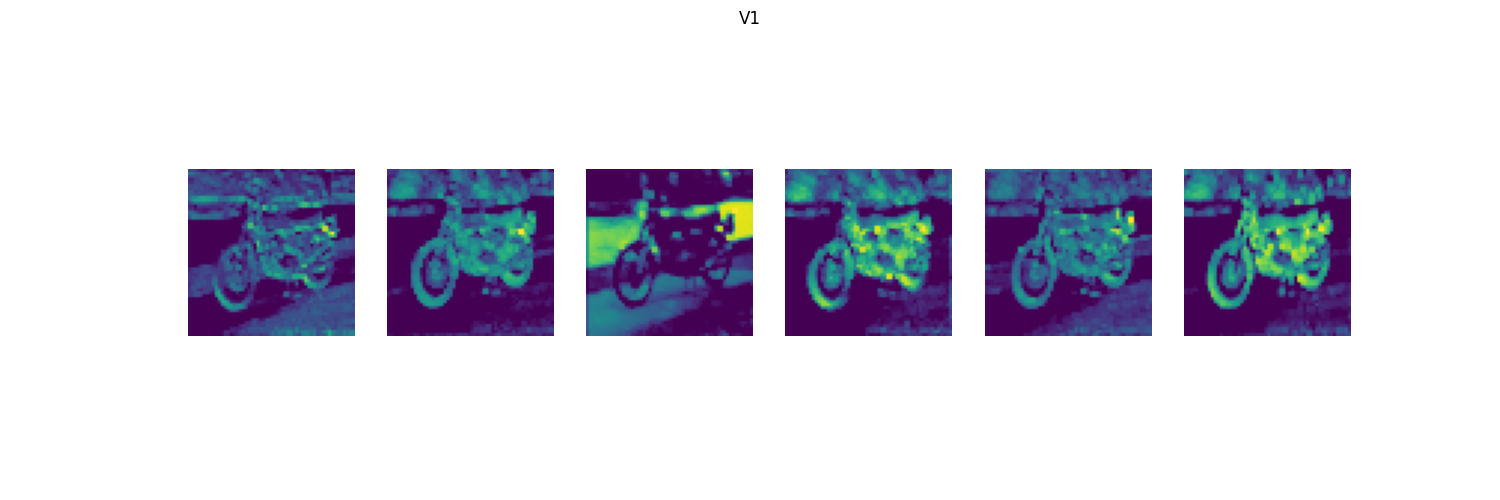
\includegraphics[width=1\linewidth]{V1_activations.png}
			\caption{V1层激活图}
		\end{minipage}
	\end{subfigure}\\
	\begin{subfigure}[t]{0.8\linewidth}
		\captionsetup{justification=centering}
		\begin{minipage}[b]{1\linewidth}
			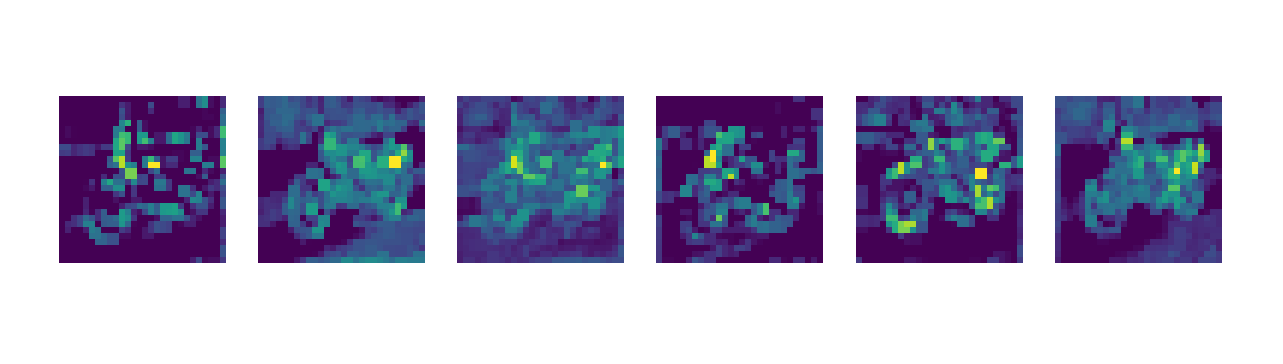
\includegraphics[width=1\linewidth]{V2_activations.png}
			\caption{V2层激活图}
		\end{minipage}
	\end{subfigure}\\
	\begin{subfigure}[t]{0.8\linewidth}
		\captionsetup{justification=centering}
		\begin{minipage}[b]{1\linewidth}
			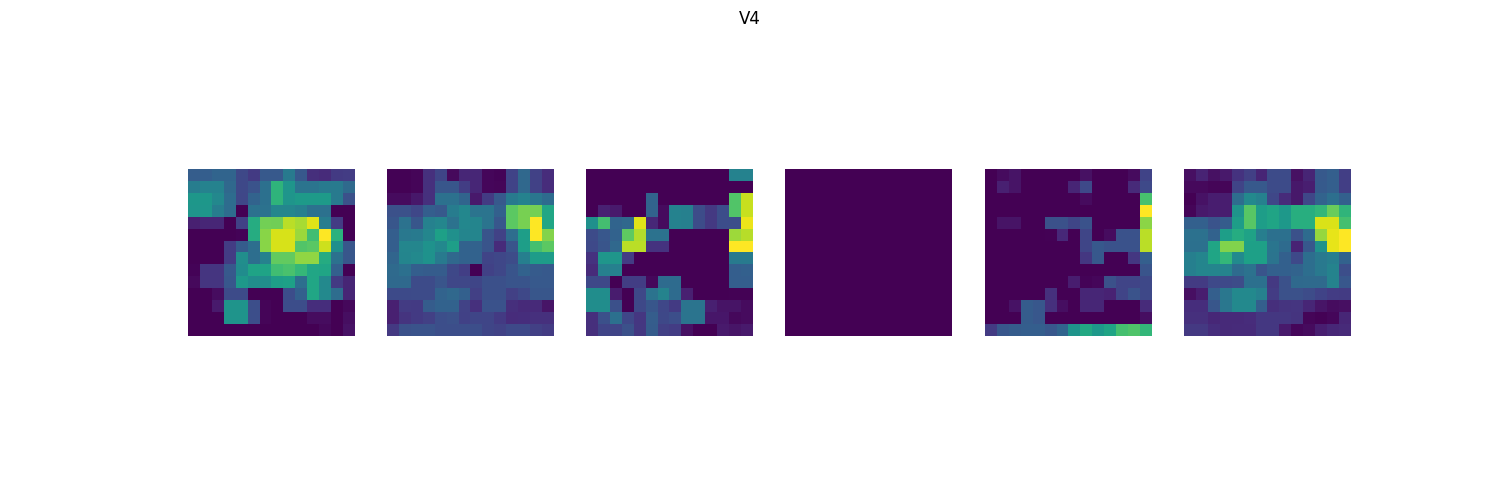
\includegraphics[width=1\linewidth]{V4_activations.png}
			\caption{V4层激活图}
		\end{minipage}
	\end{subfigure}\\
	\begin{subfigure}[t]{0.8\linewidth}
		\captionsetup{justification=centering}
		\begin{minipage}[b]{1\linewidth}
			
\includegraphics[width=1\linewidth]{IT_activations.png}
			\caption{IT层激活图}
		\end{minipage}
	\end{subfigure}
	\caption{CORnet-Z模型各层激活图}
	\label{f.cornet_z_jihuo}
\end{figure}

随着网络加深,在V2层图~\ref{f.cornet_z_jihuo}的(b)图与V4层图~\ref{f.cornet_z_jihuo}的(c)图中,激活图的结构逐渐从边缘线条过渡为较粗的区域块,表明模型开始提取更高级别的图像结构特征。

在最高层IT图~\ref{f.cornet_z_jihuo}的(d)图中,激活图整体变得更抽象,但依然可以观察到对目标核心区域的聚焦响应,表现出较强的语义抽象能力。不同通道间的激活存在差异,说明模型在高层仍保持了一定程度的特征多样性。

\subsection{引入SE机制后的激活变化}

在引入通道注意力机制后,模型的特征响应发生了明显变化。如图\ref{f.cornet_z_se_jihuo}中图(a)所示,V1层的激活图较原始模型出现了显著压缩,部分通道的响应范围明显减小,整体响应区域更加集中。

\begin{figure}[!htb]
	\centering
	\begin{subfigure}[t]{0.8\linewidth}
		\captionsetup{justification=centering}
		\begin{minipage}[b]{1\linewidth}
			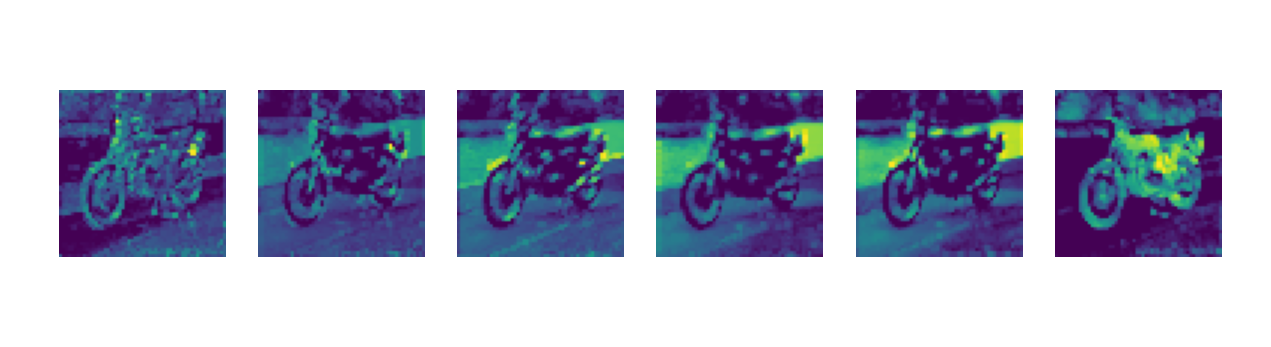
\includegraphics[width=1\linewidth]{V1_se_activations.png}
			\caption{V1层激活图}
		\end{minipage}
	\end{subfigure}\\
	\begin{subfigure}[t]{0.8\linewidth}
		\captionsetup{justification=centering}
		\begin{minipage}[b]{1\linewidth}
			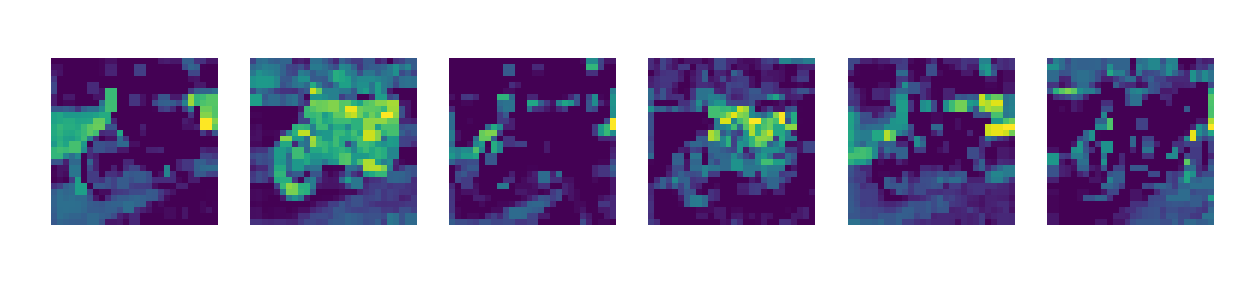
\includegraphics[width=1\linewidth]{V2_se_activations.png}
			\caption{V2层激活图}
		\end{minipage}
	\end{subfigure}\\
	\begin{subfigure}[t]{0.8\linewidth}
		\captionsetup{justification=centering}
		\begin{minipage}[b]{1\linewidth}
			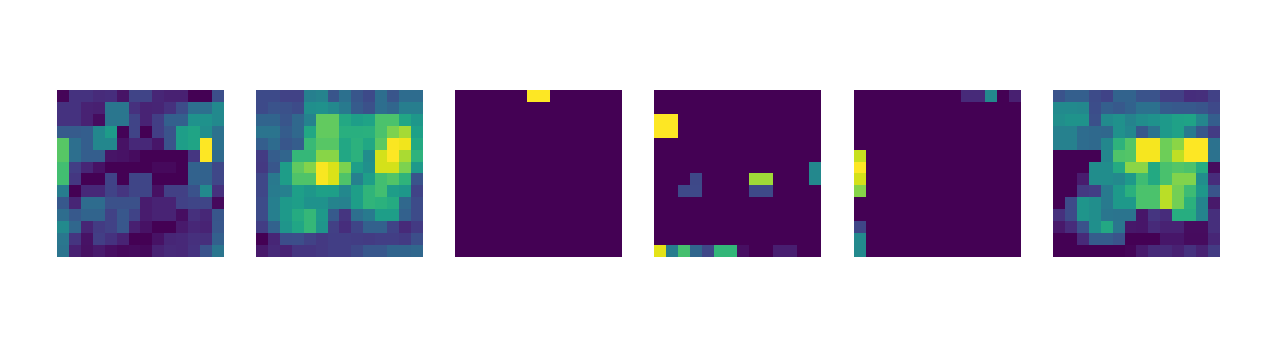
\includegraphics[width=1\linewidth]{V4_se_activations.png}
			\caption{V4层激活图}
		\end{minipage}
	\end{subfigure}\\
	\begin{subfigure}[t]{0.8\linewidth}
		\captionsetup{justification=centering}
		\begin{minipage}[b]{1\linewidth}
			
\includegraphics[width=1\linewidth]{IT_se_activations.png}
			\caption{IT层激活图}
		\end{minipage}
	\end{subfigure}
	\caption{CORnet-Z+SE模型各层激活图}
	\label{f.cornet_z_se_jihuo}
\end{figure}

V2层图\ref{f.cornet_z_se_jihuo}中图(b)表现出更零散的响应点分布,通道间响应差异增大,部分通道几乎无明显激活。

V4层图\ref{f.cornet_z_se_jihuo}中图(c)进一步体现了这种稀疏化趋势,相较于CORnet-Z模型,SE版本在此层的高响应区域数量更少,许多通道的响应接近全黑。IT层激活图层图\ref{f.cornet_z_se_jihuo}中图(d)也呈现出类似特征,尽管部分通道对图像的核心区域产生了明显响应,但整体激活的多样性有所下降。

这些变化说明,SE模块在网络中强化了部分重要通道的表达能力,同时抑制了其它通道的信息流。这种通道间的强弱选择虽然可能有助于提升分类性能,但也在一定程度上削弱了模型对图像整体结构的表达能力。

\subsection{局部目标关注能力分析}

综合观察可发现,SE模块增强了模型对图像中局部显著区域的响应能力。通过对比CORnet-Z与CORnet-Z+SE模型在V4层的激活图,可以发现注意力机制对局部目标特征的表征能力产生了显著影响。以第2个通道为例,原始模型在该通道中的激活图表现为零散分布,缺乏结构性。而在引入SE模块后,模型在相同通道上展现出更强的空间聚焦能力,激活区域更集中地覆盖于摩托车车身与轮胎等语义区域,抑制了背景部分的无效响应。

\begin{figure}[hbt]
	\centering
	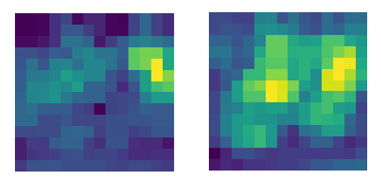
\includegraphics[width=0.4\linewidth]{V4层通道2对比图.png}
	\caption{V4层通道2对比图}
	\label{f.v4_2_act}
\end{figure}

然而,在类脑相似性方面,这种高度选择性的响应可能并不完全符合灵长类视觉皮层中多通道、分布式的响应模式。特别是在V4和IT层,SE模型在Brain-Score得分中的下降可能与激活图中体现出的稀疏性与响应单一性有关。

总体来看,原始CORnet-Z模型在各层的激活图表现出较好的层次演化特征,能够从底层边缘特征逐步整合到高层语义信息,而引入SE模块后虽然增强了判别性响应,但可能在整体特征覆盖和类脑表现方面有所取舍。
